\documentclass{sprawozdanie-agh}

\usepackage[utf8]{inputenc}
\usepackage{listings}
\usepackage{xcolor}
\usepackage{graphicx}
\usepackage{caption}
\usepackage{graphicx}
\usepackage{wrapfig}
\usepackage{subcaption}
\usepackage{accsupp}
\usepackage{array}
\usepackage{amsfonts}
\usepackage[shortlabels]{enumitem}
\usepackage{amsmath, xparse}
\usepackage{listings}

\graphicspath{ {./img/} }

\makeatletter

\begin{document}

\przedmiot{Algorytmy geometryczne}
\tytul{Laboratorium 1}
\podtytul{Ćwiczenie wprowadzające}
\kierunek{Informatyka}
\autor{Kyrylo Iakymenko\\ Czwartek 13:00 - 14:30 tydzień B}
\data{Kraków, 16 października 2023}

\stronatytulowa{}

\section{Wprowadzenie}
\subsection{Cel ćwiczenia}
\quad To ćwiczenie ma na celu zapoznanie się z metodami generacji 
losowych punktów oraz badanie metod klasyfikacji położenia punktów na płaszczyźnie 
względem prostej. 
\subsection{Położenie punktu względem prostej}

\quad Położenie punktu względem prostej będziemy wyznaczać obliczjąc
dane wyznaczniki. Wyznaczniki pozwalają określić położenie
punktu c względem prostej która jest wyznaczona przez punkty a i b.
Jeżeli wyznacznik jest większy od 0 to punkt znajduje się z lewej strony prostej, jeżeli jest mniejszy
od 0  to
punkt znajduje się po prawej stronie prostej, a jeżeli wartość wyznacznika
jest równa 0 (lub jej wartość bezwzględna $< \varepsilon$) to punkt leży na prostej.

\quad Pomimo, że
powyższe wyznaczniki są sobie równoważne to na skutek
niedoskonałości reprezentacji liczb rzeczywistych w komputerze wyniki
mogą się różnić w zależności od użytego wyznacznika.

$$
(1)\det(a, b, c)= \begin{vmatrix}
       a_{x} - c_{x} & a_{y} - c_{y} \\
       b_{x} - c_{x} & b_{y} - c_{y} 
              \end{vmatrix}.\\
              $$
              $$
(2)\det(a, b, c) = \begin{vmatrix}
    a_x & a_y & 1\\
    b_x & b_y & 1\\
    c_x & c_y & 1
\end{vmatrix}.\\
$$
\section{Zbiory testowe}
\quad Na potrzeby ćwiczenia wygenerujemy $4$ zbiory punktów losowych.
\begin{enumerate}
    \item $10^5$ losowych punktów $(x, y)$ w przestrzeni $\mathbb{R}^2$, gdzie $(x, y) \in \left[-1000,1000\right]^{2}$.
    \item $10^5$ losowych punktów $(x, y)$ w przestrzeni $\mathbb{R}^2$, gdzie $(x, y) \in \left[-10^{14},10^{14}\right]^{2}$.
    \item $1000$ losowych punktów w przestrzeni $\mathbb{R}^2$ leżących na okręgu o środku $ O = (0,0)$ i promieniu $ R = 100$.
    \item $ 1000$ losowych punktów w przestrzeni $\mathbb{R}^2$ dla $ x \in \langle -1000,1000 \rangle$ leżących na prostej wyznaczonej przez wektor $ \overrightarrow{ab}$.   
    Gdzie $ a = (-1.0, 0.0)$, $ b = (1.0, 0.1)$.
\end{enumerate}

\section{Wykresy i algorytmy generacji zbiorów}
\subsection{Wykresy wygenerowanych zbiorów}
\begin{figure}[!h]
    \centering
    \begin{subfigure}{.5\textwidth}
      \centering
      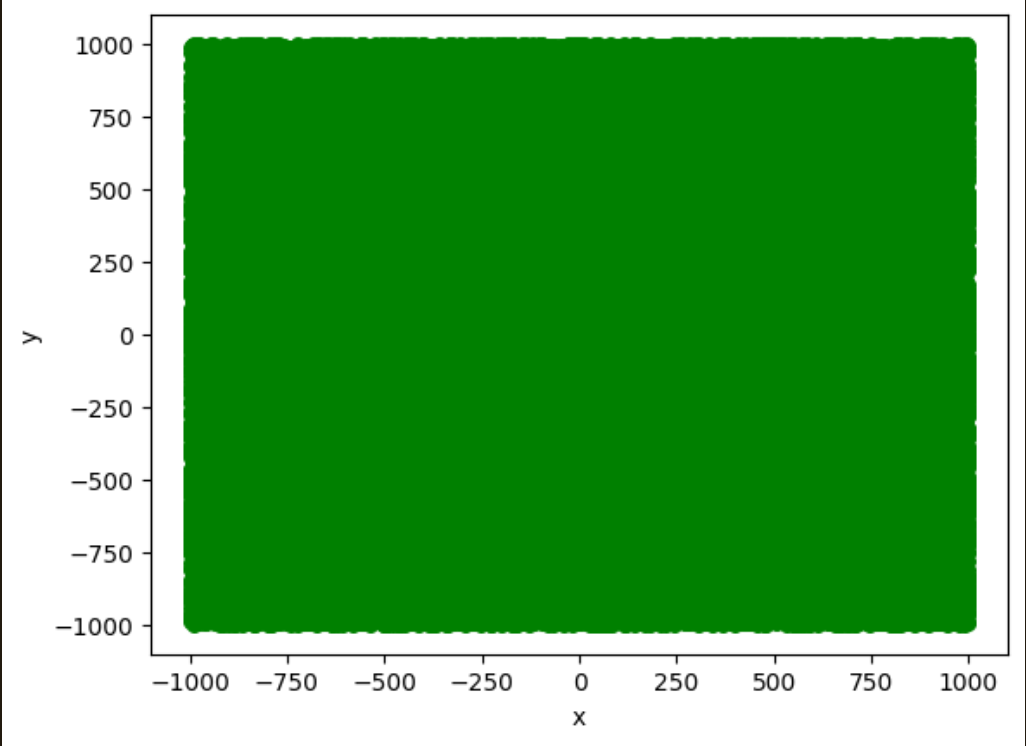
\includegraphics[width=.9\linewidth]{1.png}
      \caption*{Rys. 1: (a) $10^5$ losowych punktów $(x, y) \in \left[-1000,1000\right]^{2}$.}
      \label{fig:sub1}
    \end{subfigure}%
    \begin{subfigure}{.5\textwidth}
      \centering
      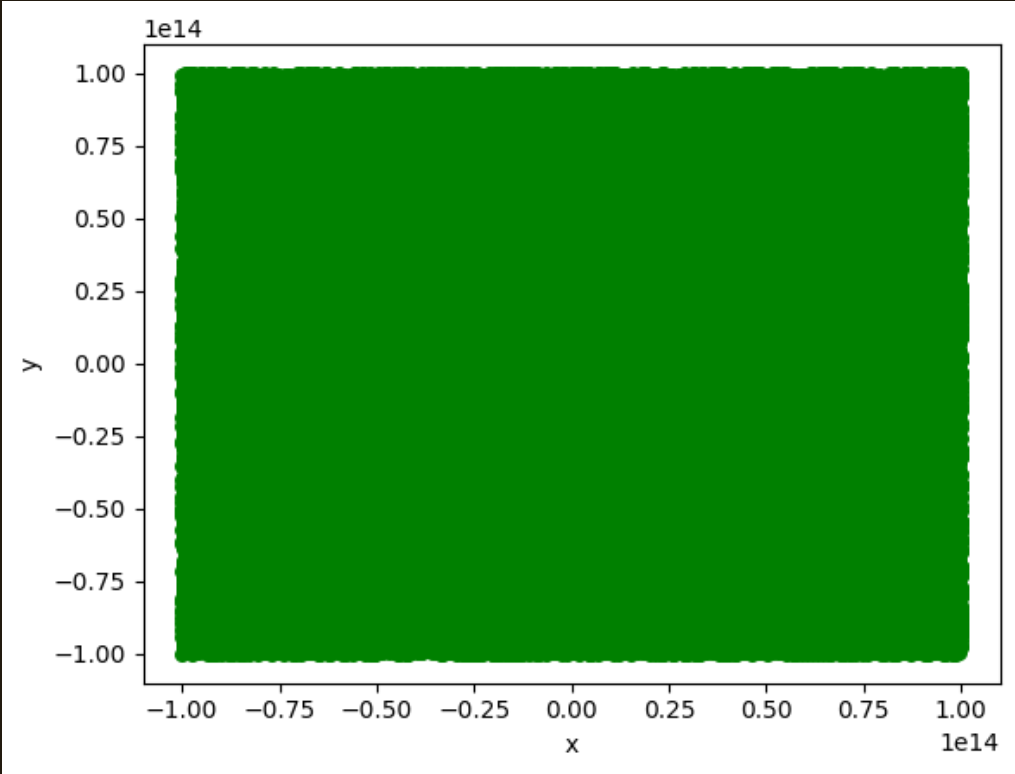
\includegraphics[width=.9\linewidth]{2.png}
      \caption*{Rys. 2: (b) $10^5$ losowych punktów $(x, y) \in \left[-10^{14},10^{14}\right]^{2}$.}
      \label{fig:sub2}
    \end{subfigure}
    \label{fig:test}
    \end{figure}
    \begin{figure}[!h]
    \centering
    \begin{minipage}{.5\textwidth}
      \centering
      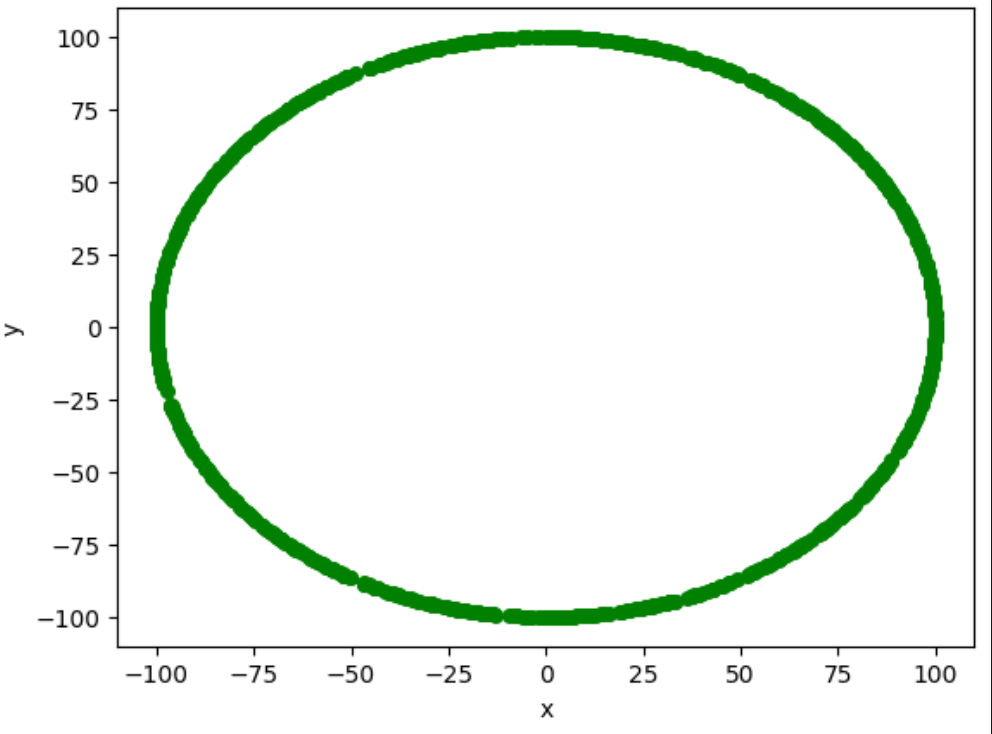
\includegraphics[width=.9\linewidth]{3.png}
      \caption*{Rys. 3: (c) $1000$ losowych punktów leżących na okręgu.}
      \label{fig:test1}
    \end{minipage}%
    \begin{minipage}{.5\textwidth}
      \centering
      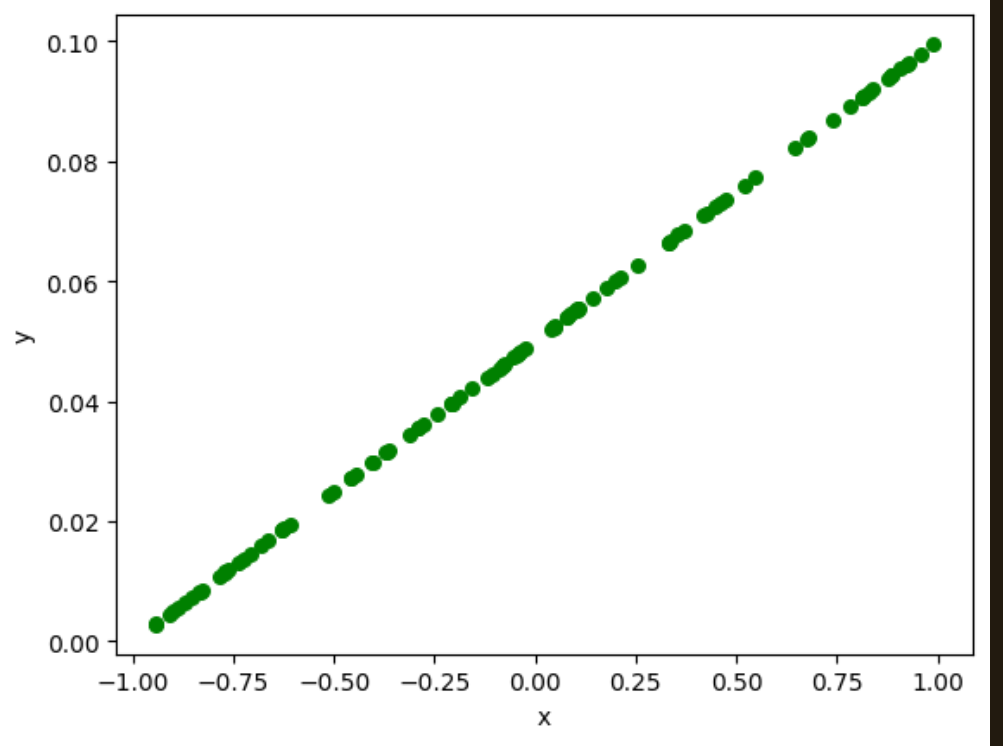
\includegraphics[width=.9\linewidth]{4.png}
      \caption*{Rys. 4: (d) $1000$ losowych punktów na prostej.}
      \label{fig:test2}
    \end{minipage}
    \end{figure}
\null
    \subsection{Algorytmy generacji zbiorów}
    \begin{enumerate}
    \item Dla zbiorów a i b. Osobna generacja każdego z $10^5$ losowych punktów.
    \item Dla zbioru c. Parametryzacja punktów na okręgu za pomocją funkcji trygonometrycznych $\sin$ i $\cos$.
    \item Dla zbioru d. Przekształcenie odcinka do postaci parametrycznej 
    $$
    l:\begin{cases}
      x = x_0 + tv_x& \smash{\raisebox{-1.6ex}{dla $\boldsymbol t \in [0,1]$.}}\\
      y = y_0 + tv_y
    \end{cases}
    $$
    A potem generowanie $t$ w podanym przedziale i dodanie odpowiednich punktów.
    \end{enumerate}
% \newpage



\section{Testy klasyfikacyjne dla różnych wartości $\varepsilon$}

\subsection{Przykładowe wykresy dla $\varepsilon = 10^{-4}$.}
\null
\begin{figure}[!ht]
    \centering
    \begin{subfigure}{.5\textwidth}
      \centering
      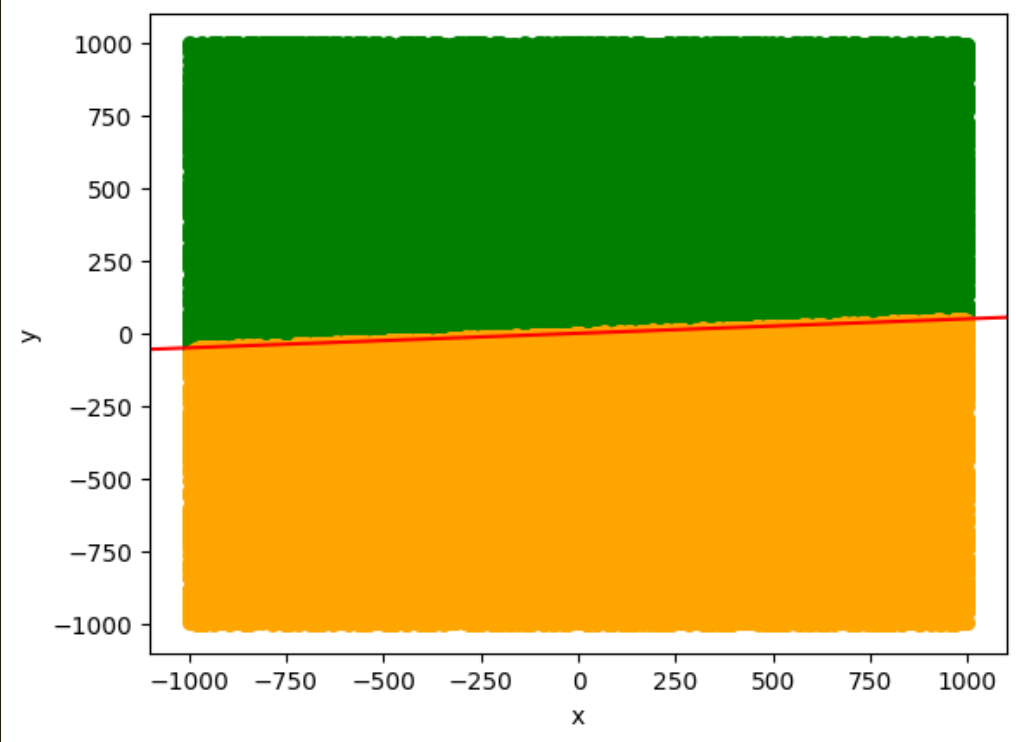
\includegraphics[width=.9\linewidth]{1k.png}
      \caption*{Rys. 5: (a) $10^5$ losowych punktów \\$(x, y) \in \left[-1000,1000\right]^{2}$.}
      \label{fig:sub1}
    \end{subfigure}%
    \begin{subfigure}{.5\textwidth}
      \centering
      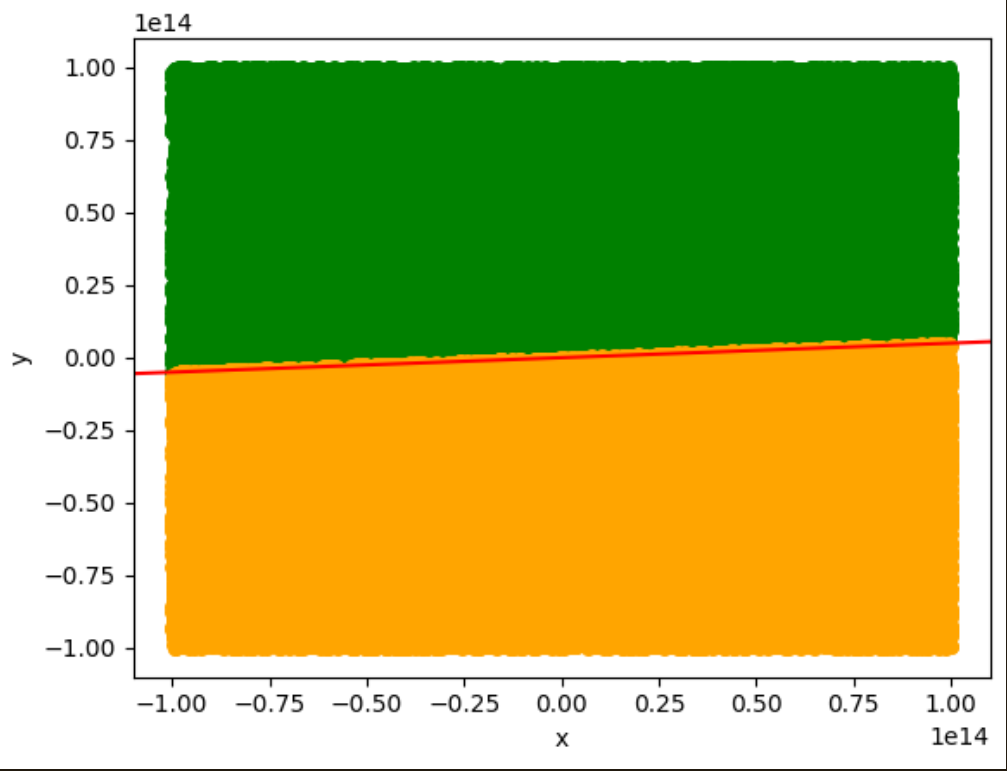
\includegraphics[width=.9\linewidth]{2k.png}
      \caption*{Rys. 6: (b) $10^5$ losowych punktów $(x, y) \in \left[-10^{14},10^{14}\right]^{2}$.}
      \label{fig:sub2}
    \end{subfigure}
    \label{fig:test}
    \end{figure}
    
    \begin{figure}[!ht]
    \centering
    \begin{minipage}{.5\textwidth}
      \centering
      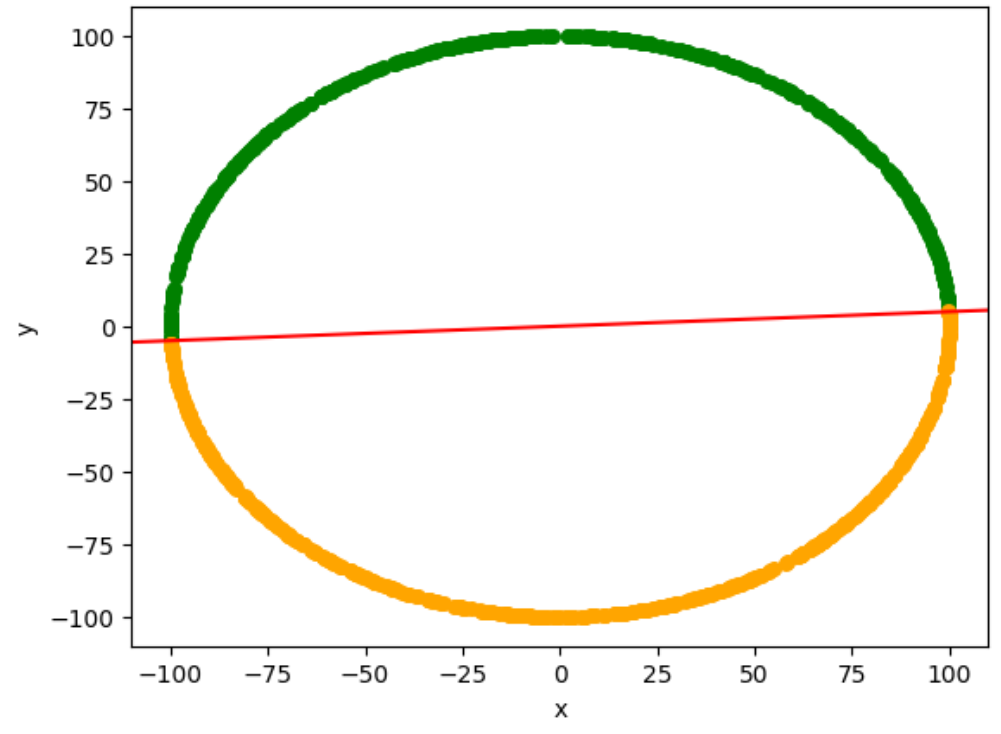
\includegraphics[width=.9\linewidth]{3k.png}
      \caption*{Rys. 7: (c) $1000$ losowych punktów leżących na okręgu.}
      \label{fig:test1}
    \end{minipage}%
    \begin{minipage}{.5\textwidth}
      \centering
      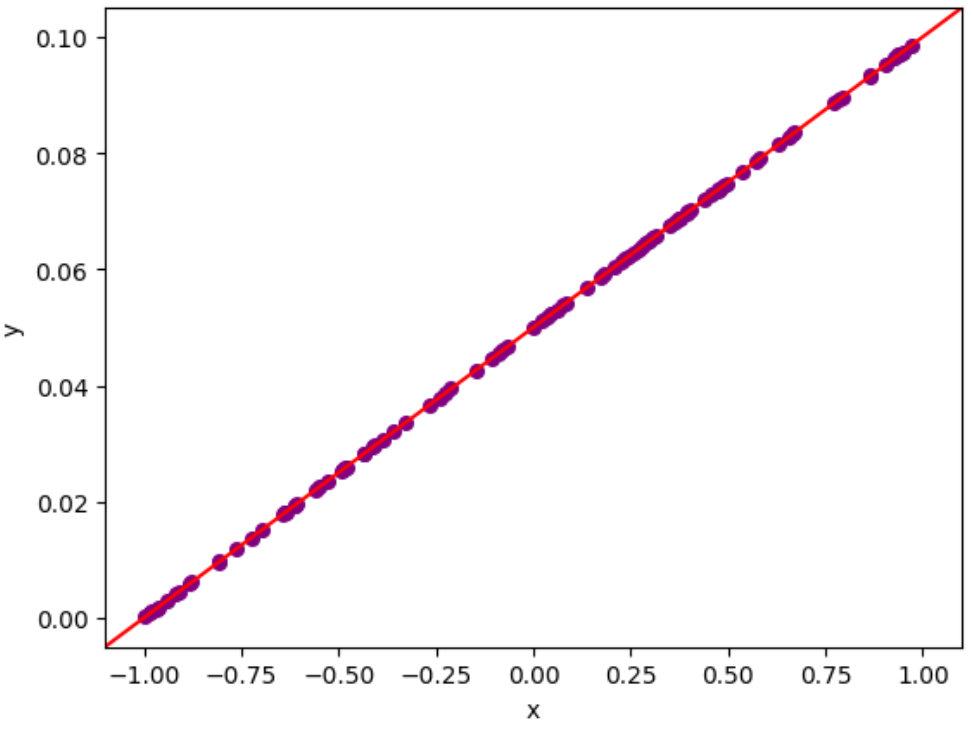
\includegraphics[width=.9\linewidth]{4k.png}
      \caption*{Rys. 8: (d) $ 1000$ losowych punktów na prostej.}
      \label{fig:test2}
    \end{minipage}
    \end{figure}
    \newpage
\subsection{Tabele}
\quad Poniżej przedstawione są tabele ilości zaklasyfikowanych punktów
 ze zbiorów \\ (a, b, c, d) ze względu na ich położenie od prostej, $\varepsilon$ tolerancje
 wartości bliskich zera oraz funkcje użytą dla obliczenia wyznacznika.\\ \\

 \begin{figure}[!hbt]
  \centering
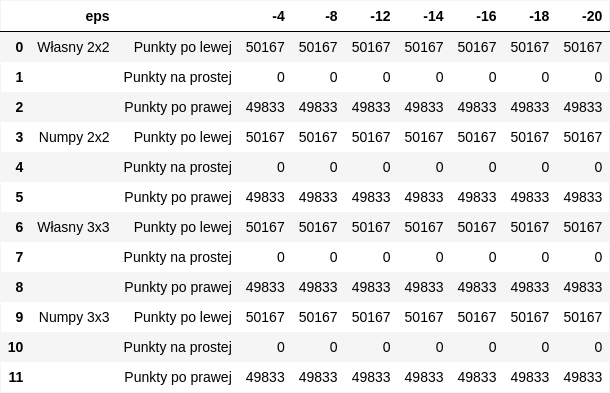
\includegraphics[scale=0.6]{eps_compar_a.png}
\caption*{Tabela 1: Wyniki dla zbioru $a$.}
 \end{figure}
 \begin{figure}[!hbt]
          \centering
    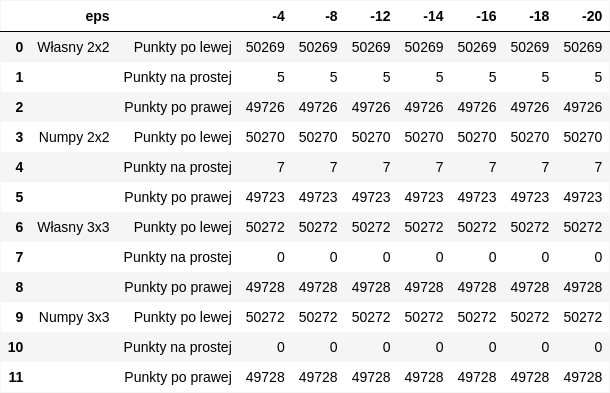
\includegraphics[scale=0.6]{eps_compar_b.png}
    \caption*{Tabela 2: Wyniki dla zbioru $b$.}
     \end{figure}
     \begin{figure}[!hbt]
          \centering
        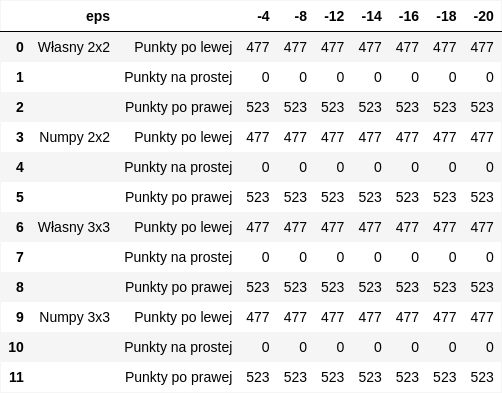
\includegraphics[scale=0.6]{eps_compar_c.png}
        \caption*{Tabela 3: Wyniki dla zbioru $c$.}
        \end{figure}
         \begin{figure}[!hbt]
          \centering
            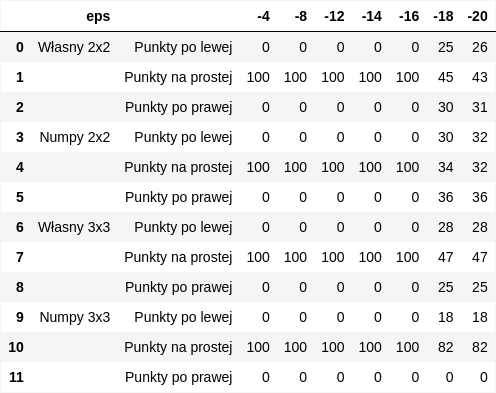
\includegraphics[scale=0.6]{eps_compar_d.png}
            \caption*{Tabela 4: Wyniki dla zbioru $d$.}
             \end{figure}
             \newpage
             \null
             \centerline{\rule{20cm}{0.4pt}}
             \newpage



             \subsection{Analiza wyników}
\begin{enumerate}
    \item \quad W zbiorze $a$ niezależnie od $\varepsilon$ widzimy brak zmian 
w ilości zaklasyfikowanych do różnych zbiorów punktów. \par
\quad Żeby zweryfikować nasze wyniki policzmy prawdopodobieństwo, że punkt w naszym zbiorze zostanie 
wylosowany w miejscu dla którego będzie zaklasyfikowany, jako należący do prostej. 
W naszych obliczeniach dla prostoty pominiemy niepewności związane z obliczeniami komputerowymi.\par
\quad Klasyfikujemy punkty do odpowiedniej grupy obliczając iloczyn wektorowy
$\overrightarrow{ab} \times \overrightarrow{ac}$, gdzie $ c = (x,y)$ jest punktem, dla którego poszukujemy wiadomości o lokalizacji względem prostej przechodzącej przez punkty $ a$ i $ b$. Metoda ta jest równoznaczna z obliczeniem wyznacznika macierzy $ 2\times2$:  

$$
(1)\det(a, b, c)= \begin{vmatrix}
       a_{x} - c_{x} & a_{y} - c_{y} \\
       b_{x} - c_{x} & b_{y} - c_{y} 
              \end{vmatrix}.
$$\par
Wiemy także, że iloczyn wektorowy $\overrightarrow{A} \times \overrightarrow{B}$ można także obliczyć ze wzoru: 
$$
\overrightarrow{A} \times \overrightarrow{B} = ||A|| \cdot ||B|| \cdot \sin{\theta}.
$$
\quad Gdzie $\sin{\theta}$ to kąt pomiędzy wektorami $\overrightarrow{A}$ i $\overrightarrow{B}$.\\
Wybierzmy teraz dla konkretnego punktu $c$ takie $a$ i $b$ na prostej, żeby 
\begin{enumerate}
    \item Dla $A = \overrightarrow{ab}, ||{A}|| = 1$.
    \item $\sin{\theta} = 1$, gdzie $\theta$ jest kątem pomiędzy $\overrightarrow{ab}$ i $\overrightarrow{ac}$ (wektor $\overrightarrow{ac}$ jest prostopadły do naszej prostej i do wektora $\overrightarrow{ab}$).
\end{enumerate}
Wtedy nasz iloczyn $$\overrightarrow{A} \times \overrightarrow{B} = ||A|| \cdot ||B|| = 1 \cdot ||B|| = ||B||.$$
\quad I pytanie klasyfikacji punktu jako należacego do prostej sprowadza się do sprawdzenia czy $||B|| < \varepsilon$.
Dla zbioru $a$ długość prostej o równaniu $y = \frac{1}{20}x - 1$ na całym zbiorze $(-1000, 1000)$ jest równa 
$$
    \sqrt{(y(1000) - y(-1000))^2 + (1000 + 1000)^2} = \sqrt{10 ^ 4 + 4 \cdot 10^6} = \sqrt{4,01 \cdot 10^6} \approx 2 \cdot 10^3.
$$
Pole obszaru na którym punkty będą klasyfikowane jako należące do prostej zate wynosi
$$
    2 \cdot 2 \cdot 10^3 \cdot \varepsilon = 4 \cdot 10^3 \cdot \varepsilon.
$$
Teraz w porównaniu do całkowitego pola naszego zbioru
$$
    \frac{4 \cdot 10^3 \cdot \varepsilon}{(1000 - (-1000))^2}=
    \frac{4 \cdot 10^3 \cdot \varepsilon}{4 \cdot 10^6} =  10^{-3} \cdot \varepsilon.
$$
\quad Patrząc na ten wynik dla $\varepsilon = 10^{-4}$ nie jest zadziwiające to, że 
żaden z $10^5$ punktów nie został zakwalifikowany jako leżący na prostej. Gdzyż prawdopodobieństwo 
wylosowania takiego punktu to tylko $10^{-7}$.
\item \quad Dla zbioru b widzimy, że dla wszystkich $10^{-20} < \varepsilon < 10^5$ dostajemy ten sam wynik 
, czego też warto było się spodziewać gdzyż stosując metodę opisaną w poprzednim podpunkcie dostajemy 
prawdopodobieństwo wylosowania punktu leżącego na prostej 
$$
    \frac{4 \cdot 10^{14} \cdot \varepsilon}{(10^{14} - (-10^{14}))^2}=
    \frac{4 \cdot 10^{14} \cdot \varepsilon}{4 \cdot 10^{28}} =  10^{-14} \cdot \varepsilon.
$$
\quad Czyli nawet dla $\varepsilon = 10^5$ prawdopodobieństwo, że conajmniej jeden z $10^5$ punktów zostanie zaklasyfikowany 
do prostej to około $10^{-4}$.\par
\quad Natomiast obserwujemy też specyficzne dla wyznacznika $2\times 2$ zachowanie, 
a mianowicie niezależnie od $\varepsilon$ pewna stała ilość punktów zostaje zaklasyfikowana jako leżąca na prostej. 
Prawdopodobnie to jest związane z tym, że wyznacznik $2\times 2$ jest mniej precyzyjny 
w porównaniu do wyznacznika $3\times 3$.
\item \quad Dla zbioru c widzimy podobną sytuację. Dla $\varepsilon > 10^{-2}$ 
każde zmniejszenie $\varepsilon$ powoduje ogromne zmiany w wynikach, ale podalsze zwiększenie precyzji 
nie ma żadnego efektu na wynikach.

\item \quad Dla zbioru d zmniejszenie $\varepsilon$ ma największe znaczenie ze wszystkich. 
Nawet przejście pomiędzy $\varepsilon = 10^{-16}$ do $\varepsilon = 10^{-18}$ ma ogromne znaczenie 
na ilości punktów zakwalifikowanych do prostej.
\end{enumerate}

\section{Porównywanie czasów klasyfikacji dla różnych funkcji obliczających wyznacznik}
\quad Poniżej przedstawiona jest tabela średniego czasu klasyfikacji na 
zbiorze testowym specjalnie dla tego celu (zbiór ma ogromną ilość punktów).
$10^6$ losowych punktów $(x, y)$ w przestrzeni $\mathbb{R}^2$, gdzie $(x, y) \in \left[-10^{14},10^{14}\right]^{2}$.
\begin{lstlisting}
    test_set = generate_uniform_points(-10^4, 10^4, 10 ** 6)
\end{lstlisting}
\begin{figure}[htb]
    \centering 
    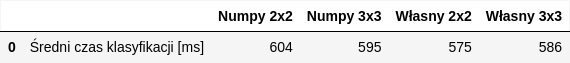
\includegraphics[scale=0.6]{wyz.png}\par
    \caption*{Tabela 5: Czasy klasyfikacji na zbiorze testowym. }
\end{figure}
\quad Widzimy ogromne różnice w czasach klasyfikacji naszego zbioru dla różnych wyznaczników. 
Najbardziej oczywistą różnicą jest różnica pomiędzy wyznacznikami napisanymi ręcznie, a 
funkcjami bibliotecznymi, z których ostatnie demonstrują dużo gorsze czasy. 
Prawdopodobnie możemy zaobserwować takie zjawisko dlatego, że funkcje biblioteczne implementują dużo większy zakres 
narzędzi, przez co pod czas wielokrotnego wywołania tej samej funkcji są wolniejsze w porównaniu do 
kilku prostych operacji arytmetycznych, którymi są nasze funkcje liczące wyznacznik. 
\section{Testy precyzji float64 i float32}
\quad Na poniższym wykresie jest przedstawiona tabela ilości 
zaklasyfikowanych do prostej punktów w zależności od precyzji zminnej (float32, float64) i 
$\varepsilon$.
zbiorze testowym specjalnie dla tego celu (zbiór punktów na prostej).
$ 10^4$ losowych punktów w przestrzeni $\mathbb{R}^2$ dla $ x \in \langle -1000,1000 \rangle$ leżących na prostej wyznaczonej przez wektor $ \overrightarrow{ab}$.   
    Gdzie $ a = (-1.0, 0.0)$, $ b = (1.0, 0.1)$.
\\
\begin{figure}[hbt]
    \centering
    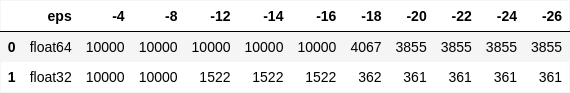
\includegraphics[scale=0.6]{eps.png}
    \caption*{Tabela 6: Porównanie precyzji float64 i float 32.}
\end{figure}
\par
\quad Patrząc na porównanie precyzji float64 z float32, możemy dojść do wniosku, 
że float64 daje (jak wypadało się spodziewać) dużo większą precyzje obliczeń. 
Widoczna jest poważna różnica w obliczeniach już dla $\varepsilon = 10^{-12}$. 
Dlatego na potrzeby algorytmów geometrycznych zalecane jest 
używanie float64.
\section{Podsumowanie}
\quad Porównując ilość zaklasyfikowanych punktów dla różnych $\varepsilon$ dostaliśmy róźne wyiniki 
dla róznych metod obliczenia wyznacznika. 
Klasyfikacja punktów ze zbiorów a oraz c dawała podobne wyniki niezależnie od użytej
funkcji liczenia wyznacznika czy $\varepsilon$. Spowodowane jest to tym, że
istnieje bardzo małe prawdopodobieństwo, iż punkt będzie znajdował się
dokładnie na prostej, z dokładnością do użytej tolerancji. W podpunkcie
b wybór epsilona nie miał znaczenia jednak wybór wyznacznika już tak.
Jest to spowodowane dużymi odległościami pomiędzy punktami. Operacja klasyfikacji punktów wymaga jednak
dużej precyzji, która jest tracona z powodu dużych wartości które są
generowane. Z tego możemy dojść do wniosku, że użycie wyznaczników $3 \times 3$ daje 
nam większą precyzje w obliczeniach, a też patrząc na wyniki porównania wydajności funkcji 
liczących wyznacznik, są wykonywane tak samo szybko, jak i funkcje liczenia wyznacznika $2 \times 2$.
\par
\quad Patrząc na porównanie precyzji float64 z float32, możemy dojść do wniosku, 
że float64 daje (jak wypadało się spodziewać) dużo większą precyzje obliczeń. 
Widoczna jest poważna różnica w obliczeniach już dla $\varepsilon = 10^{-12}$. 
Na tej podstawie na potrzeby algorytmów geometrycznych zalecane jest 
używanie float64.
\par
\quad We wszystkich testach i porównaniach statystycznych dostaliśmy 
wyniki, które zgadzały się z wartościami teoretycznymi. Na tej 
podstawie możemy dojść do wniosku, że w obliczeniach nie było poważnych 
błędów i ćwiczenie było wykonane poprawnie.

\end{document}
